
\section*{Problema P11.38}

\renewcommand*\thesection{11.38}
\numberwithin{equation}{section}
\numberwithin{figure}{section}

\begin{center}
    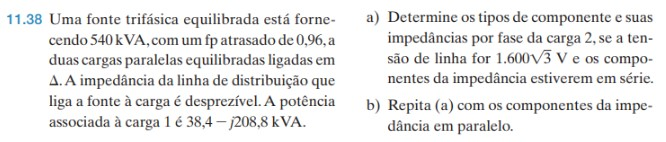
\includegraphics[scale=1.0]{P11.38.jpg}
\end{center}

\subsection*{(a)}

A fonte trifásica fornece uma potência total $S = 540 \un{kVA}$, com um fator de potência atrasado de $FP = 0.96$. 
O fator de potência atrasado significa que a carga é indutiva, possuindo um ângulo de fase $\phi < 0$. \\
Sabemos que o fator de potência é definido como   

\begin{equation}\label{eq:11.38.1}
    FP = \frac{P}{ |S| }
\end{equation}

Isolando $P$ e substituindo, temos   

\[ P = (FP)|S| \logo P = 518400 \un{W} \]

Além disso, temos que a potência aparente $S$ se relaciona com as potências ativa $P$ e reativa $Q$ através de

\begin{equation}\label{eq:11.38.2}
    S^2 = P^2 + Q^2
\end{equation}

Isolando $Q$ e substituindo, temos

\[ Q = \sqrt{S^2 - P^2} \logo Q = 151200 \un{VA}_R \]

Portanto, a potência total fornecida pela fonte é

\[ S_T = 518400 \un{W} + 151200 \un{VA}_R \]

Como a carga 1 dissipa $S_1 = 38.4 -j208.8 \un{kVA}$, e sabemos que

\[ S_2 = S_T - S_1 \]

Temos 

\[ S_2 = 480 + j360 \un{kVA} \]

Além disso, como as cargas são trifásicas e equilibradas, temos que cada fase recebe exatamente $\frac{1}{3}$ da potência da carga.
Assim, cada fase de $S_2$ recebe 

\[ S_{2/\phi} = 160 + j120 \un{kVA} \]

\begin{figure}[hb]
    \centering
    \caption{(a) Componentes da carga em série. (b) Componentes da carga em paralelo}
      \centering
      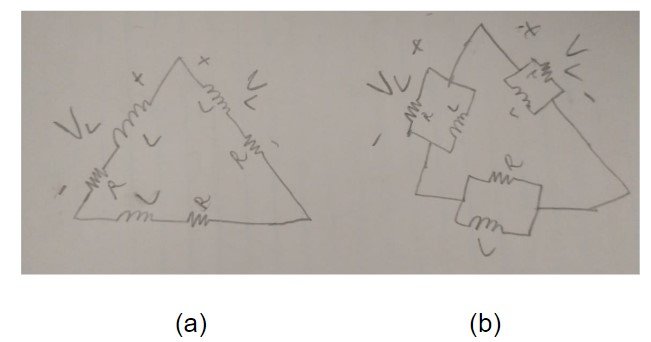
\includegraphics[scale=0.5]{P11.38-Item(a,b).jpg} \\
    \label{fig:11.38.1}
\end{figure}

No caso dos componentes da carga estarem em série, como mostra a Figura \ref*{fig:11.38.1} (a), temos 

\begin{equation}\label{eq:11.38.3}
    S_{2/\phi} = \frac{ |V_L|^2}{Z^*}
\end{equation}

Isolando $Z$ em \eqref{eq:11.38.3},  

\[ Z_s = \left(\frac{ |V_L|^2}{ S_{2/\phi} }\right)^* = \left(\frac{ |1600\sqrt{3}|^2}{ 160000 + j120000 }\right)^*  \]

\[ Z_s = \left(\frac{7680000}{ 160000 + j120000 }\right)^* = (30.72 - j23.04)^* = 30.72 + j23.04 \un{$\Omega$} \]

Assim, usando $L = \frac{X_L}{j\omega}$ e assumindo a fonte trifásica operando em $f =60 \un{Hz}$, temos os componentes em série dados por

\[ \boxed{R = 30.72 \un{$\Omega$} \quad , \quad L = 61.1 \un{mH} } \]

\subsection*{(b)}

Agora usamos os componentes em paralelo, como mostra a Figura \ref*{fig:11.38.1} (b). Note que o resistor $R$ irá dissipar totalmente
a parte real da potência, enquanto o idutor $L$ está associado totalmente à parte imaginária da potência. Assim, podemos fazer  

\[ R = \left(\frac{ |V_L|^2}{ Re\;\{S_{2/\phi}\}  }\right)^* \]

\[ R = \left(\frac{ |1600\sqrt{3}|^2}{ 160000  }\right)^* = 48 \un{$\Omega$} \]

Agora para a parte imaginária associada ao indutor, 

\[ X_L = \left(\frac{ |V_L|^2}{ Im\;\{S_{2/\phi}\}  }\right)^* \]

\[ X_L = \left(\frac{ |1600\sqrt{3}|^2}{ j120000  }\right)^* =(-j 64)^* = j64 \un{$\Omega$} \]

Novamente usando $L = \frac{X_L}{j\omega}$, identificamos a indutância de L, obtendo

\[ \boxed{R = 48 \un{$\Omega$} \quad , \quad L = 169.8 \un{mH} } \]


